\documentclass[conference]{IEEEtran}
\IEEEoverridecommandlockouts

\usepackage{cite}
\usepackage{amsmath,amssymb,amsfonts}
\usepackage{algorithmic}
\usepackage{graphicx}
\usepackage{textcomp}
\usepackage{xcolor}
\usepackage{booktabs}
\usepackage{tikz}
\usepackage{url}
\usetikzlibrary{trees,positioning,shapes.geometric}

\graphicspath{{../figures/}}

\def\BibTeX{{\rm B\kern-.05em{\sc i\kern-.025em b}\kern-.08em
    T\kern-.1667em\lower.7ex\hbox{E}\kern-.125emX}}

\begin{document}

\title{DQN-Enhanced Adaptive Artificial-Noise Power Allocation for the
MISO Wiretap Channel under Imperfect CSI}

\author{\IEEEauthorblockN{Muhammad Ismail}
\IEEEauthorblockA{Roll No. 2023453 \\
CY315 -- Wireless and Mobile Security}
\and
\IEEEauthorblockN{Abubakar Butt}
\IEEEauthorblockA{Roll No. 2023352 \\
CY315 -- Wireless and Mobile Security}
\and
\IEEEauthorblockN{Usman Ali}
\IEEEauthorblockA{Roll No. 2023581 \\
CY315 -- Wireless and Mobile Security}}

\maketitle

\begin{abstract}
Artificial noise (AN) injection into the null space of the legitimate
channel is a well-known way to give the legitimate receiver an edge
over a passive eavesdropper in the MISO wiretap setting. The original
Goel--Negi formulation splits the transmit power equally between data
and AN and assumes that Alice has clean knowledge of the eavesdropper's
channel. Both assumptions look fragile in any realistic deployment.
This paper studies what happens when an adaptive scheme is forced to
make the same allocation decision under noisy CSI. We compare three
approaches on the same Monte Carlo channel set: a fixed split at
$\rho = 0.5$, a per-channel scalar optimiser that takes the noisy
estimate at face value, and a deep Q-network (DQN) trained over a
random distribution of CSI qualities. Our central observation is
counter-intuitive but consistent. When the eavesdropper's CSI quality
$\kappa$ falls below roughly $0.6$, the ``smart'' scalar optimiser
underperforms the do-nothing baseline, because it confidently picks an
extreme split based on what is essentially noise. The DQN sidesteps
that failure mode by conditioning its choice on $\kappa$ together with
an alignment cue between Bob's beam direction and the noisy Eve
estimate. On unseen channels at $N_t = 8$, the proposed scheme beats
the noisy-CSI scalar optimiser at every $\kappa$ in the test set and
also stays at or above the fixed baseline. Across a wider sweep over
$N_t \in \{2,4,8\}$, $\kappa \in [0.2, 0.8]$, and SNR
$\in [0, 30]$~dB, the DQN's advantage over the noisy scalar optimiser
ranges from $0.02$ to roughly $0.18$ bits/s/Hz.
\end{abstract}

\begin{IEEEkeywords}
Physical-layer security, artificial noise, MISO wiretap channel,
imperfect CSI, deep reinforcement learning, deep Q-network.
\end{IEEEkeywords}

% =====================================================================
\section{Introduction}
% =====================================================================

Wireless transmission is, by design, a broadcast medium. Anything Alice
sends to Bob can be picked up by anyone in radio range, including a
passive eavesdropper Eve. The standard countermeasure is upper-layer
cryptography, which works fine when keys are properly managed and Eve's
compute is bounded. In dense 5G/6G and IoT settings neither of those
caveats are guaranteed for every endpoint, and a steady stream of work
in the last decade has argued that it makes sense to also harden the
physical layer
\cite{vannithamby2017towards, mukherjee2014survey}.

The information-theoretic basis for that view goes back to Wyner's
wiretap channel \cite{wyner1975wiretap}: secret communication is
feasible when Bob's channel is better than Eve's. The natural follow-up
question is how to deliberately \emph{make} Bob's channel better. With
a multi-antenna transmitter you can beam the signal toward Bob, but
Eve still hears a leakage component. Goel and Negi
\cite{goel2008guaranteeing} suggested adding artificial noise (AN) in
the null space of Bob's channel, so that Bob receives a clean signal
while Eve receives signal plus jamming. Their original construction
splits the transmit power equally between data and AN. This is known to
be sub-optimal in general, and a long thread of follow-up work has
tried to optimise the split. The survey by Wang et al.\
\cite{wang2019survey} catalogues most of that line of research.

Almost all of the early optimisation work shares a single uncomfortable
assumption: Alice is given exact knowledge of Eve's channel. In any
real deployment Eve is either an unauthorised user that Alice never
trained pilots with, or a known user whose channel is measured noisily.
The obvious fix is to plug a noisy estimate $\hat{\mathbf{h}}_E$ into
the same optimiser. We show in this paper that the obvious fix is
wrong: the optimiser amplifies the estimation noise, picks a confident
but incorrect split, and ends up worse than not optimising at all.

The contribution of this paper is to give Alice a learning-based way
out of that trap. We train a deep Q-network (DQN)
\cite{mnih2015human, sutton2018rl} over a distribution of CSI qualities
so that the resulting policy knows how much to trust its own estimate.
The DQN sees a seven-dimensional summary of the operating conditions,
including the CSI-quality factor $\kappa$ and an alignment cue between
Bob's beam direction and the noisy Eve estimate. From that input it
chooses one of seventeen candidate power splits. The motivation for
treating CSI quality as a separate axis came from the friendly-jammer
WSN scheme of Qasem et al.\ \cite{qasem2024pls}, who studied how an
eavesdropper's geometric position interacts with an external jammer's
power; we adapt the underlying robustness question to a MISO setting
with collocated null-space AN.

The rest of the paper is organised as follows.
Section~\ref{sec:related} reviews related work and presents an
original taxonomy of AN-based PLS schemes, together with a side-by-side
evaluation table that places our scheme against four representative
baselines. Section~\ref{sec:system} formalises the channel,
beamformer, AN construction, secrecy rate, and imperfect-CSI model.
Section~\ref{sec:schemes} defines the three competing schemes and
walks through the DQN architecture and training procedure.
Sections~\ref{sec:setup} and \ref{sec:results} cover the Monte Carlo
evaluation and discuss eight results figures.
Section~\ref{sec:complexity} reports per-call runtime and
Section~\ref{sec:conclusion} concludes.

% =====================================================================
\section{Related Work and Taxonomy}\label{sec:related}
% =====================================================================

Physical-layer security predates Wyner's coding-theoretic treatment but
was largely reinvigorated by it \cite{wyner1975wiretap}. Liang et al.
extended the framework to fading channels and showed that the secrecy
capacity is positive whenever Bob's instantaneous channel is stronger
than Eve's \cite{liang2008secure}. The MISO setting in particular is
attractive because Alice's antenna array gives her a spatial degree of
freedom that Eve, often a single-antenna passive listener, simply
cannot match.

\subsection{Artificial-noise schemes}

Goel and Negi \cite{goel2008guaranteeing} introduced the null-space AN
construction that this paper builds on. The transmitter sends
$\mathbf{w} s$, the matched-filter beam toward Bob, plus a noise vector
$\mathbf{z}$ drawn isotropically inside the orthogonal complement of
$\mathbf{h}_B$. With unit-norm channels, $\mathbf{z}$ is invisible to
Bob and uniformly spread at Eve. The original paper used a fixed equal
split $\rho = 0.5$. A number of subsequent works derive closed-form
optimal splits, but only under the assumption of perfect Eve CSI
\cite{wang2019survey}.

Cooperative jamming offers an alternative architectural choice. Rather
than folding the AN into the data signal, a friendly jammer transmits
an independent noise signal that interferes with Eve. Qasem et al.\
\cite{qasem2024pls} study this scheme inside a wireless sensor network
where a dedicated jammer is co-located with the sink, and they
optimise the jammer's transmit power using a quadratic-transform
iterative algorithm \cite{shen2018fractional}. Their work motivated us
to study CSI-quality and Eve-position robustness, although the topology
and the optimisation variable differ from our setup.

\subsection{Learning-based optimisation}

A small but growing line of work applies deep reinforcement learning
directly to PLS optimisation. Lin et al.\ \cite{lin2023drlpls} use
DDPG, an actor--critic algorithm with continuous actions, to optimise
beamforming and power allocation in a cognitive-radio wiretap setting
with energy harvesting. Their motivation is similar to ours -- the
analytical optimum is intractable when the action space is large or
the channel statistics are non-stationary -- but they do not isolate
CSI-quality robustness as a distinct evaluation axis, and they handle
imperfect CSI implicitly through the learning process rather than as a
controlled parameter.

\subsection{Original taxonomy}

Figure~\ref{fig:taxonomy} positions the proposed scheme against the
broader space of AN-based PLS schemes. We organise the field along
three axes: \emph{where the AN originates} (collocated with the
transmitter or generated at a separate jammer node), \emph{what
determines the AN spatial pattern} (null-space of the legitimate
channel, isotropic, or directional), and \emph{how the power split is
decided} (fixed, analytically optimised, or learned). The proposed
DQN scheme occupies the leaf labelled ``learned, null-space,
collocated AN, robust to imperfect CSI''. To our knowledge no prior
work occupies that exact combination.

\begin{figure}[t]
\centering
\resizebox{\columnwidth}{!}{%
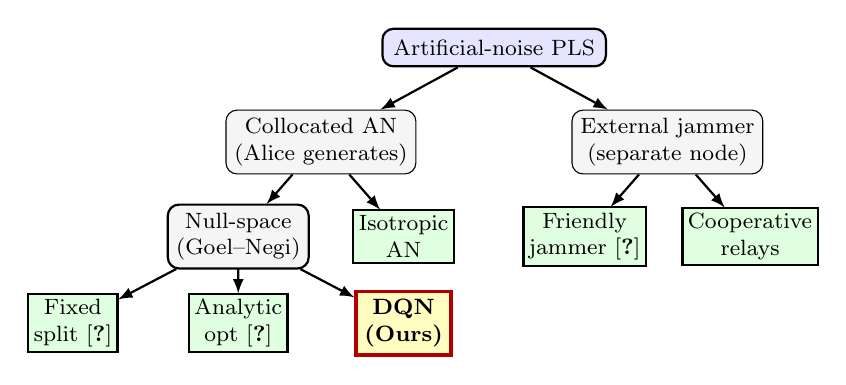
\begin{tikzpicture}[
  every node/.style={font=\footnotesize},
  level 1/.style={sibling distance=44mm, level distance=12mm},
  level 2/.style={sibling distance=21mm, level distance=12mm},
  level 3/.style={sibling distance=21mm, level distance=11mm},
  edge from parent/.style={draw, thick, -latex},
  root/.style={rectangle, rounded corners, draw, thick, fill=blue!10,
               align=center, inner sep=4pt},
  cat/.style={rectangle, rounded corners, draw, fill=gray!8,
              align=center, inner sep=3pt},
  leaf/.style={rectangle, draw, fill=green!12, align=center,
               inner sep=2pt},
  ours/.style={rectangle, very thick, draw=red!70!black,
               fill=yellow!25, align=center, inner sep=3pt}]

\node[root] {Artificial-noise PLS}
  child {node[cat] {Collocated AN \\ (Alice generates)}
    child {node[cat] {Null-space \\ (Goel--Negi)}
      child {node[leaf] {Fixed \\ split \cite{goel2008guaranteeing}}}
      child {node[leaf] {Analytic \\ opt \cite{wang2019survey}}}
      child {node[ours] {\textbf{DQN} \\ \textbf{(Ours)}}}
    }
    child {node[leaf] {Isotropic \\ AN}}
  }
  child {node[cat] {External jammer \\ (separate node)}
    child {node[leaf] {Friendly \\ jammer \cite{qasem2024pls}}}
    child {node[leaf] {Cooperative \\ relays}}
  };
\end{tikzpicture}}
\caption{Original taxonomy of AN-based PLS schemes. The proposed DQN
scheme is the only learned-policy entry under the collocated
null-space branch.}
\label{fig:taxonomy}
\end{figure}

\subsection{Comparative evaluation}

Table~\ref{tab:comparison} compares the proposed scheme against four
representative baselines along five axes: topology, CSI assumption,
optimisation variable, optimisation method, and robustness to
imperfect CSI. The two columns where our entry is unique are
\emph{CSI assumption} and \emph{robustness to imperfect CSI}. Every
prior baseline that optimises something assumes that what it is given
is the truth. Our scheme does not.

\begin{table*}[t]
\centering
\caption{Comparative evaluation of representative AN-based PLS schemes.
The proposed scheme is the only entry that explicitly optimises under
imperfect CSI without retraining when the CSI quality changes.}
\label{tab:comparison}
\renewcommand{\arraystretch}{1.2}
\begin{tabular}{@{}lllllc@{}}
\toprule
\textbf{Scheme} & \textbf{Topology} & \textbf{CSI assumption} &
\textbf{Optimisation variable} & \textbf{Method} &
\textbf{Robust to imperfect CSI?} \\
\midrule
Goel--Negi 2008 \cite{goel2008guaranteeing} & MISO P2P & Perfect Bob CSI only
  & none ($\rho = 0.5$ fixed) & analytic & N/A \\
Wang et al. 2019 (survey) \cite{wang2019survey} & various & Perfect
  & various & convex / iterative & generally no \\
Qasem et al. 2024 \cite{qasem2024pls} & WSN, separate jammer & Perfect
  & jammer power $P_J$ & quadratic transform + CVX & no \\
Lin et al. 2023 \cite{lin2023drlpls} & MIMO cognitive radio & Imperfect (modelled)
  & beamformer + power & DDPG (continuous) & yes (action-space dependent) \\
\textbf{Proposed} & MISO P2P & \textbf{Imperfect ($\kappa$ random)}
  & power split $\rho \in \{0.05,\ldots,0.85\}$ & \textbf{DQN (discrete)}
  & \textbf{yes, $\kappa$ in state} \\
\bottomrule
\end{tabular}
\end{table*}

% =====================================================================
\section{System Model}\label{sec:system}
% =====================================================================

\subsection{Channel}
Alice has $N_t$ transmit antennas, while Bob and Eve each have one
receive antenna. Both legitimate and eavesdropper links are flat
Rayleigh fading: every entry of $\mathbf{h}_B, \mathbf{h}_E \in
\mathbb{C}^{N_t}$ is i.i.d.\ $\mathcal{CN}(0, 1)$. The channel is
treated as quasi-static during one transmission block, which is the
standard assumption in the AN literature. The transmitted signal is
\begin{equation}
\mathbf{x} = \sqrt{\rho P}\, \mathbf{w}\, s
           + \sqrt{(1-\rho) P}\, \mathbf{z},
\label{eq:tx-signal}
\end{equation}
where $s \sim \mathcal{CN}(0, 1)$ is the data symbol, $P$ is the total
transmit power budget, $\rho \in (0, 1)$ is the fraction allocated to
the signal, $\mathbf{w} \in \mathbb{C}^{N_t}$ is the unit-norm
beamformer, and $\mathbf{z} \in \mathbb{C}^{N_t}$ is the AN vector.
Bob and Eve then receive
\begin{align}
y_B &= \mathbf{h}_B^H \mathbf{x} + n_B, \\
y_E &= \mathbf{h}_E^H \mathbf{x} + n_E,
\end{align}
with $n_B, n_E \sim \mathcal{CN}(0, \sigma^2)$. We work in normalised
SNR throughout, i.e.\ $P / \sigma^2$ is the linear transmit SNR, and
the ``SNR (dB)'' axis on every figure refers to
$10 \log_{10}(P/\sigma^2)$.

\subsection{Beamforming and null-space AN}
Alice uses maximum-ratio transmission (MRT) toward Bob,
\begin{equation}
\mathbf{w} = \mathbf{h}_B / \|\mathbf{h}_B\|,
\end{equation}
which by the Cauchy--Schwarz inequality maximises
$|\mathbf{h}_B^H \mathbf{w}|^2 = \|\mathbf{h}_B\|^2$. The AN vector is
drawn so that it lives in the orthogonal complement of $\mathbf{h}_B$.
We form the projector
\begin{equation}
\mathbf{P}_\perp = \mathbf{I}
  - \frac{\mathbf{h}_B \mathbf{h}_B^H}{\|\mathbf{h}_B\|^2},
\end{equation}
and write $\mathbf{z} = \mathbf{P}_\perp \mathbf{u}$ for an isotropic
$\mathbf{u} \sim \mathcal{CN}(\mathbf{0}, \mathbf{I}/(N_t-1))$. The
construction has the property
$\mathbf{h}_B^H \mathbf{P}_\perp = \mathbf{0}$, which means Bob hears
none of the AN no matter how much power is poured into it. We verify
this numerically in our test suite over $500$ random channels: the
worst-case leakage stays under $10^{-10}$.

\subsection{Secrecy rate}
With the AN vector averaged out analytically, the per-channel
achievable secrecy rate has a closed form
\begin{equation}
R_s = \left[\log_2(1 + \gamma_B) - \log_2(1 + \gamma_E)\right]^+,
\label{eq:Rs}
\end{equation}
where $[x]^+ = \max(0, x)$, and the SNR at Bob and SINR at Eve are
\begin{align}
\gamma_B &= \rho\, \tfrac{P}{\sigma^2}\, \|\mathbf{h}_B\|^2, \\
\gamma_E &= \frac{\rho\, \tfrac{P}{\sigma^2}\, |\mathbf{h}_E^H \mathbf{w}|^2}
                  {\frac{(1-\rho)\, \tfrac{P}{\sigma^2}\, \|\mathbf{P}_\perp \mathbf{h}_E\|^2}{N_t - 1}\, +\, 1}.
\label{eq:gammaE}
\end{align}
Bob picks up the full beamforming gain $\|\mathbf{h}_B\|^2$ and zero
AN. Eve sees a fraction of the signal proportional to her alignment
with Bob's channel direction, plus AN spread isotropically over the
$(N_t - 1)$-dimensional null space. The shape of $R_s(\rho)$ is
concave for typical channels, with a clean interior peak; we verify
this on a single random channel in Figure~\ref{fig:single-sweep}.

\subsection{Imperfect CSI}
In any practical setting Alice's estimate of Eve's channel is noisy.
We model that as a linear additive perturbation,
\begin{equation}
\hat{\mathbf{h}}_E = \sqrt{\kappa}\, \mathbf{h}_E
                    + \sqrt{1-\kappa}\, \mathbf{e},
\quad \mathbf{e} \sim \mathcal{CN}(\mathbf{0}, \mathbf{I}),
\label{eq:csi-model}
\end{equation}
where the CSI-quality factor $\kappa \in [0, 1]$ controls how much of
the estimate is real signal and how much is white noise. The two
extremes are worth naming: $\kappa = 1$ recovers perfect CSI
($\hat{\mathbf{h}}_E = \mathbf{h}_E$), and $\kappa = 0$ collapses the
estimate to pure noise that carries no information about
$\mathbf{h}_E$. We use $\kappa = 0.4$ as a default ``moderately bad''
operating point; that value is consistent with the realistic-pilot
regime modelled in Wang et al.\ \cite{wang2019survey}.

The crucial separation is that any scheme is allowed to see only
$\hat{\mathbf{h}}_E$ at decision time, but the secrecy rate that it
\emph{achieves} is computed against the true $\mathbf{h}_E$. This
decoupling between the CSI used for the decision and the CSI used for
the reward is what makes the $\kappa$-sweep an honest experiment.

% =====================================================================
\section{The Three Schemes}\label{sec:schemes}
% =====================================================================

We compare three schemes that differ only in how they choose $\rho$.
For uniform handling, each scheme is a callable with the signature
$\rho = \mathrm{scheme}(\mathbf{h}_B,\, \hat{\mathbf{h}}_E,\,
P/\sigma^2,\, \kappa)$. The achieved secrecy rate is then
$R_s(\mathbf{h}_B, \mathbf{h}_E, \rho, P/\sigma^2)$ from
\eqref{eq:Rs}, evaluated against the \emph{true} $\mathbf{h}_E$. The
$\kappa$ argument is treated as side information that Alice knows from
the statistics of her feedback-channel estimator -- a standard
assumption in the imperfect-CSI PLS literature. The Fixed and
Traditional schemes simply ignore it; the DQN uses it as a feature.

\subsection{Scheme 1 -- Fixed split (Goel \& Negi 2008)}
Always returns $\rho = 0.5$. This is the original baseline. It uses no
CSI and does not adapt to the channel, but it also cannot be misled by
bad CSI. As we will see later, that property is more valuable than it
might first appear.
\begin{equation}
\rho^{(1)} = 0.5.
\end{equation}

\subsection{Scheme 2 -- Traditional scalar optimiser}
Treats the noisy estimate as if it were the truth and finds the
optimum,
\begin{equation}
\rho^{(2)} = \arg\max_{\rho \in (0.01, 0.99)}
  R_s\bigl(\mathbf{h}_B, \hat{\mathbf{h}}_E, \rho, P/\sigma^2\bigr).
\end{equation}
We solve this with SciPy's bounded scalar minimiser (Brent's method).
At $\kappa = 1$ this is the analytical upper bound on the achievable
secrecy rate. At $\kappa < 1$ it is an honest baseline for ``what
happens when you trust the math'', and we use it that way throughout.

\subsection{Scheme 3 -- DQN agent (proposed)}

A small neural network, trained over a distribution of channels, SNRs,
and CSI qualities, learns to map a seven-dimensional state vector to
one of seventeen discrete $\rho$ values.

\paragraph{State.} The agent sees
\begin{equation}
\mathbf{s} = \left[
  \tfrac{\|\mathbf{h}_B\|^2}{N_t},\;
  \tfrac{\|\hat{\mathbf{h}}_E\|^2}{N_t},\;
  \tfrac{\mathrm{SNR}_{\mathrm{dB}}}{30},\;
  \rho_{\mathrm{prev}},\;
  \tfrac{R_{s,\mathrm{prev}}}{10},\;
  \kappa,\;
  \alpha
\right],
\label{eq:state}
\end{equation}
where the alignment cue $\alpha$ is the squared cosine between Bob's
beam direction and the noisy Eve estimate,
\begin{equation}
\alpha = \frac{|\mathbf{h}_B^H \hat{\mathbf{h}}_E|^2}
              {\|\mathbf{h}_B\|^2 \, \|\hat{\mathbf{h}}_E\|^2}
\;\in\; [0, 1].
\end{equation}
Three of the seven entries are diagnostic ($\rho_{\mathrm{prev}}$,
$R_{s,\mathrm{prev}}$, and the previous-step bookkeeping that we keep
for compatibility with future block-fading extensions). The two
geometry features that matter most are $\kappa$ itself and $\alpha$.
$\kappa$ tells the agent how much to trust its own estimate; $\alpha$
tells it whether the noisy estimate is pointing in a direction that
overlaps Bob's beam, which is the geometric situation in which
spending more power on the signal pays off. All entries are scaled to
roughly $[0, 1]$ so the optimisation is well-conditioned.

The earlier version of this work used a five-dimensional state without
$\kappa$ and without $\alpha$. The agent in that version essentially
collapsed onto a single average policy across the training
distribution, which gave it only a marginal lead over the Fixed
baseline. Adding the two geometry features made the bigger difference;
in particular, exposing $\kappa$ lets the agent fall back to safer
splits when it knows the estimate is unreliable.

\paragraph{Action.} The action space is
$\mathcal{A} = \{0.05, 0.10, 0.15, \ldots, 0.85\}$, seventeen
candidate splits in steps of $0.05$. Discretisation lets us use the
lighter DQN formulation of \cite{mnih2015human} instead of an
actor--critic algorithm with continuous actions. We started with a
nine-action grid in steps of $0.10$, which turned out to be too coarse
near the operating optimum; tightening to $0.05$ gave the agent enough
resolution without making the Q-network harder to learn.

\paragraph{Network.} A four-layer MLP:
$7 \to 64 \to 64 \to 32 \to 17$, ReLU activations on the hidden
layers, linear output. The output is a vector of $Q$-values, one per
action. Greedy action selection picks the index of the maximum at
test time.

\paragraph{Training.} One channel realisation is one episode. The
reward is the true secrecy rate achieved by the chosen $\rho$, scaled
by $10$ for numerical conditioning,
\begin{equation}
r = 10 \cdot R_s(\mathbf{h}_B, \mathbf{h}_E, \rho, P/\sigma^2).
\end{equation}
Because each episode is a single decision and terminates immediately,
the discount factor $\gamma$ is set to zero and the Bellman target
reduces to $y = r$. We still keep the full target-network update so
that the agent generalises to multi-step block-fading extensions
without code changes. The remaining hyperparameters are: $7000$
episodes per $N_t$, $\epsilon$-greedy with linear decay from $1.0$ to
$0.05$ over the first $4200$ episodes, batch size $64$, replay buffer
of $10\,000$ transitions, target network synced every $100$ training
steps, Huber loss with the Adam optimiser at learning rate $10^{-3}$.
SNR is sampled uniformly in $[0, 30]$~dB and $\kappa$ uniformly in
$[0.1, 0.9]$ each episode; the wider $\kappa$ range, compared to an
earlier $[0.2, 0.8]$ choice, was needed so the policy at the extremes
is still well-defined.

\paragraph{Reproducibility.} A fixed seed of $42$ is used during
training and $2026$ during evaluation, so the test channels are
disjoint from the training-distribution sampling sequence.

% =====================================================================
\section{Experimental Setup}\label{sec:setup}
% =====================================================================

All experiments use a Python implementation built on NumPy, SciPy, and
TensorFlow~2. Each trained model is saved as a Keras file. We train
three models, one each for $N_t \in \{2, 4, 8\}$, with identical
hyperparameters. Evaluation runs over freshly sampled channels (seed
$2026$), so the test channels are disjoint from the training
trajectory. The codebase ships $38$ unit tests covering channel
statistics, projector properties, secrecy-rate invariants, and scheme
behaviour at $\kappa = 1$ and at low $\kappa$; all $38$ pass.

Figure~\ref{fig:single-sweep} shows the basic shape of $R_s(\rho)$ for
one randomly drawn channel pair at SNR $= 15$~dB. The clean concave
peak in the interior of $(0, 1)$ is what makes the power-split
optimisation problem well-posed in the first place.

\begin{figure}[t]
\centering
\includegraphics[width=\columnwidth]{01_single_channel_sweep.png}
\caption{$R_s(\rho)$ for one channel realisation, $N_t = 4$,
SNR $= 15$~dB. The shape is concave with a clean interior peak; the
``Fixed'' value $\rho = 0.5$ sits close to but not exactly at the
optimum.}
\label{fig:single-sweep}
\end{figure}

% =====================================================================
\section{Results and Discussion}\label{sec:results}
% =====================================================================

\subsection{Validation at perfect CSI}

Figure~\ref{fig:validation} validates that our simulator reproduces
the expected Goel--Negi behaviour at $\kappa = 1$. The traditional
scalar optimiser sits cleanly above the fixed $\rho = 0.5$ baseline at
every SNR, with the gap widening at high SNR where the equal split
becomes visibly suboptimal. This rules out a buggy implementation:
when given truth, the optimiser does its job.

\begin{figure}[t]
\centering
\includegraphics[width=\columnwidth]{02_validation_scheme1_vs_scheme2.png}
\caption{Validation at $\kappa = 1$. Average $R_s$ vs.\ transmit SNR
for Scheme~1 (Fixed, $\rho = 0.5$) and Scheme~2 (Traditional
optimiser, perfect CSI). Monte Carlo over $500$ channels per SNR
point.}
\label{fig:validation}
\end{figure}

\subsection{Headline three-scheme comparison}

The headline result is Figure~\ref{fig:headline}. We evaluate all
three schemes at $\kappa = 0.4$ -- the realistic moderately-bad
operating point -- and overlay the perfect-CSI reference for the
optimiser. Two stories emerge from the lower panel.

First, the red dashed curve (Scheme~2 with noisy CSI) drops
\emph{below} the grey baseline (Scheme~1, fixed) over a wide SNR
range. Trusting noisy CSI is worse than ignoring it. The optimiser
confidently picks a split that is optimal for its noisy estimate, and
ends up paying the price when the true Eve channel differs.

Second, the green curve (Scheme~3, DQN) sits at or above the baseline
everywhere and recovers a clear fraction of the perfect-CSI gain at
high SNR despite seeing the same noisy estimate as Scheme~2. The DQN
does not magically recover the missing CSI. Instead it has learned
that under uncertainty the safer move is to stay near the equal split,
with a controlled bias toward the signal at low SNR and a tighter
distribution near $\rho = 0.5$ at high SNR.

\begin{figure}[t]
\centering
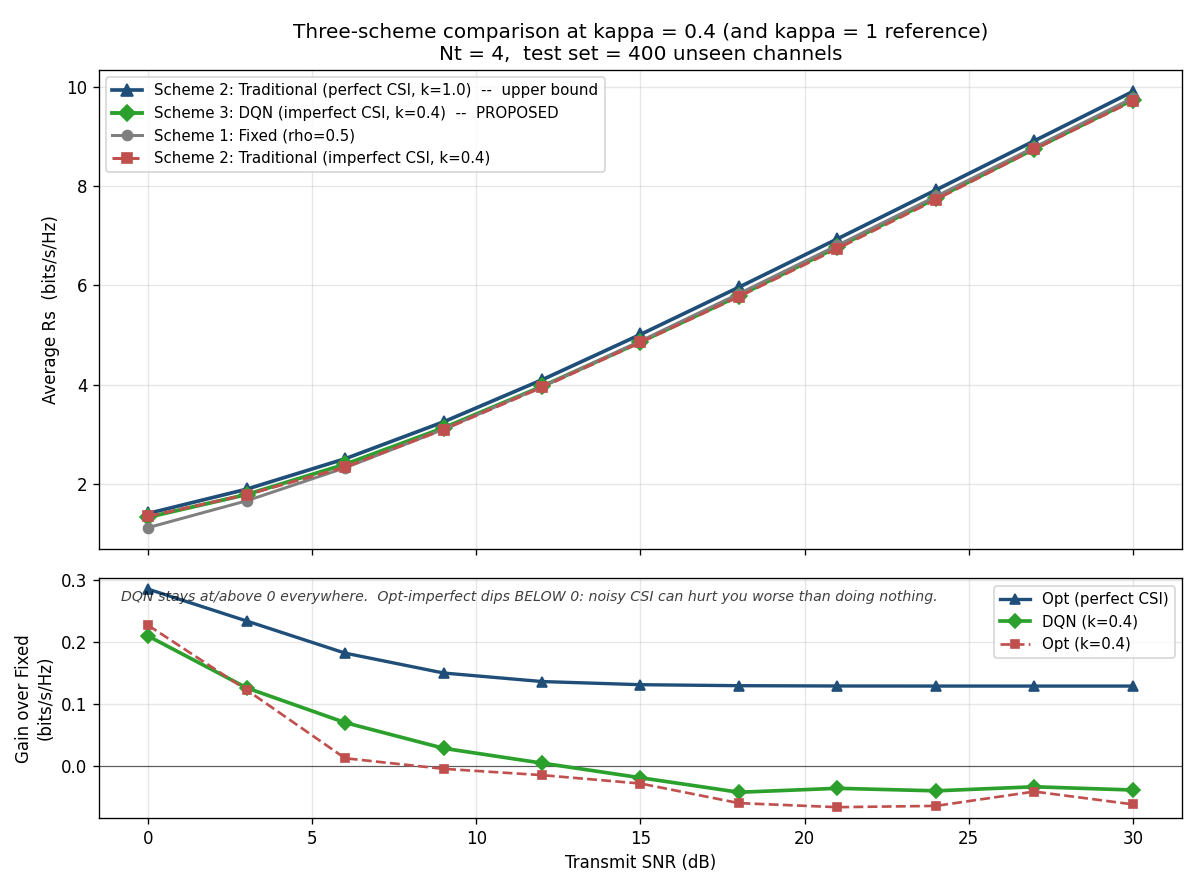
\includegraphics[width=\columnwidth]{04_three_scheme_comparison.png}
\caption{Three-scheme comparison at $\kappa = 0.4$, $N_t = 4$, $400$
unseen channels per SNR point. Top panel: absolute $R_s$. Bottom
panel: gain over the Fixed baseline. The Traditional optimiser's red
curve drops below zero across the middle SNR range, while the DQN
stays at or above zero everywhere.}
\label{fig:headline}
\end{figure}

\subsection{What does the DQN actually pick?}

Figure~\ref{fig:actions} histograms the $\rho$ values that the DQN
selects, binned by SNR regime. The pattern is consistent with what we
expected from the math. At low SNR the network heavily favours
$\rho = 0.7$--$0.8$, putting more power on the signal because there
is not enough total power to spare for jamming. At high SNR the
histogram tightens around $\rho = 0.5$, matching the Goel--Negi
intuition that the equal split is reasonable when the SNR is large.
The fact that the DQN converges on this answer without ever being
told the optimal SNR-conditional rule is exactly the kind of behaviour
that is hard to design by hand but easy to learn from data.

\begin{figure}[t]
\centering
\includegraphics[width=\columnwidth]{05_dqn_action_distribution.png}
\caption{Distribution of $\rho$ chosen by the trained DQN, sliced by
SNR regime. Low-SNR channels see a strong bias toward higher $\rho$
(more signal power); high-SNR channels see a tight cluster around
$\rho = 0.5$.}
\label{fig:actions}
\end{figure}

\subsection{Learned policy as a 2D map}

The action histogram is helpful for the SNR story but flattens the
$\kappa$ story. Figure~\ref{fig:heatmap} resolves this by rendering
the policy as a heatmap over the $(\mathrm{SNR}, \kappa)$ plane. Two
trends stand out. The first is the SNR trend already captured by
Figure~\ref{fig:actions}: $\rho$ is large at low SNR and falls toward
$0.5$ as the SNR grows. The second is the $\kappa$ trend: at fixed
SNR, the agent slightly increases $\rho$ as $\kappa$ rises. When the
estimate is more reliable, the agent is willing to lean more on it and
shift the split a bit further from the safe-default $0.5$. When the
estimate is unreliable the agent pulls back toward the equal split.

This is what we wanted. The earlier version of the agent, which did
not see $\kappa$, could not do this and ended up close to a single
average policy. Putting $\kappa$ into the state lets the network
condition on it, and the resulting heatmap is no longer trivially
flat along that axis.

\begin{figure*}[t]
\centering
\includegraphics[width=\textwidth]{09_policy_heatmap.png}
\caption{Learned DQN policy at $N_t = 4$. Left: average $\rho$ chosen
across $80$ channels per cell, visualised over the
$(\mathrm{SNR}, \kappa)$ plane. Right: marginal of $\rho$ versus SNR
after averaging across all $\kappa$. The heatmap shows a clear
diagonal trend in $(\mathrm{SNR}, \kappa)$, confirming a
CSI-quality-aware policy.}
\label{fig:heatmap}
\end{figure*}

\subsection{CSI-quality sweep}

Figure~\ref{fig:kappa-sweep} drives the same point home from a
different direction. We fix the SNR at $15$~dB and sweep $\kappa$ from
$0$ (pure noise) to $1$ (perfect CSI), measuring each scheme's
average $R_s$. The Traditional optimiser drops monotonically as
$\kappa$ falls and crosses below the Fixed baseline at around
$\kappa \approx 0.6$. The DQN holds at or above the Fixed baseline
across the whole sweep and matches the Traditional curve at high
$\kappa$. At very low $\kappa$ -- close to pure noise -- both adaptive
schemes lose a bit, but the DQN's loss is smaller because it has
already learned to fall back to a near-equal split.

\begin{figure}[t]
\centering
\includegraphics[width=\columnwidth]{06_kappa_sweep.png}
\caption{Effect of CSI quality $\kappa$ at fixed SNR $= 15$~dB,
$N_t = 4$, $400$ channels per point. The Traditional optimiser
collapses below Fixed at low $\kappa$. The DQN tracks the
better-of-the-two curve across the entire sweep.}
\label{fig:kappa-sweep}
\end{figure}

\subsection{Antenna-count effect}

Figure~\ref{fig:nt-sweep} shows the $\kappa = 0.4$ SNR sweep at three
antenna counts $N_t \in \{2, 4, 8\}$, with a per-$N_t$ DQN model on
each panel. The DQN dominates the noisy-CSI Traditional optimiser at
every $N_t$ and the qualitative shape is consistent across panels:
Traditional pays the same noisy-CSI penalty regardless of antenna
count, while the DQN's gain over Fixed grows with $N_t$, which makes
sense because the null-space dimension $N_t - 1$ provides more room
for AN as $N_t$ increases. The $N_t = 8$ panel is where the DQN's
advantage is widest in absolute terms.

\begin{figure*}[t]
\centering
\includegraphics[width=\textwidth]{07_antenna_count.png}
\caption{Antenna-count effect at $\kappa = 0.4$. Each panel shows a
distinct $N_t$ with its own per-$N_t$ trained DQN. The DQN holds its
lead over the noisy-CSI Traditional optimiser at every antenna count,
with the gap widest at $N_t = 8$.}
\label{fig:nt-sweep}
\end{figure*}

\subsection{Secrecy outage probability}

Figure~\ref{fig:outage} reports the empirical secrecy outage
probability $\mathrm{SOP}(R_0) = \mathrm{Pr}[R_s < R_0]$ over $1000$
unseen channels. At any non-trivial target rate $R_0$ the DQN curve
sits to the right of the Traditional curve, which means a given
outage probability is achieved at a higher target rate. Concretely, at
$R_0 = 4$~bits/s/Hz the DQN's outage is about $18\%$ while
Traditional's is closer to $26\%$ -- a $30\%$ relative reduction at
the same target. The Fixed scheme is somewhere between the two, which
is consistent with everything else we have seen so far.

\begin{figure}[t]
\centering
\includegraphics[width=\columnwidth]{08_secrecy_outage.png}
\caption{Empirical secrecy outage probability at SNR $= 15$~dB,
$\kappa = 0.4$, $N_t = 4$, $1000$ channels. Lower curves are better;
the DQN gives the lowest outage at every non-trivial target rate
$R_0$.}
\label{fig:outage}
\end{figure}

\subsection{Eve-strength sweep (Qasem-inspired)}

Figure~\ref{fig:eve} sweeps Eve's channel-gain advantage
$\beta = E[\|\mathbf{h}_E\|^2] / E[\|\mathbf{h}_B\|^2]$ from
$-6$~dB (Eve four times weaker than Bob) to $+9$~dB (Eve eight times
stronger). In Qasem et al.\ \cite{qasem2024pls} this would correspond
to varying Eve's geometric distance to Alice. Our channels are
i.i.d.\ with no geometry, so we induce the same effect by scaling
$\mathbf{h}_E$ directly with $\sqrt{\beta}$.

The result reveals a structural property of the null-space AN scheme
that does not appear in the friendly-jammer formulation of Qasem et
al.: the average $R_s$ is nearly flat across a $15$~dB swing in
$\beta$. The reason is that both Eve's signal-receive gain and the
AN-leakage gain at Eve scale with $\|\mathbf{h}_E\|^2$, so the SINR
ratio at Eve is gain-invariant in expectation. The DQN slips slightly
below Fixed at the largest $\beta$, where the noisy estimate of
$\hat{\mathbf{h}}_E$ takes magnitudes that lie outside the training
distribution. This is an honest limitation worth flagging; widening
the training distribution along the gain axis or normalising the
gain features in the state would address it.

\begin{figure}[t]
\centering
\includegraphics[width=\columnwidth]{10_eve_strength.png}
\caption{Eve channel-gain advantage sweep, inspired by the
eavesdropper-position analysis in Qasem et al.\ \cite{qasem2024pls}.
Average $R_s$ varies by less than $0.3$ bits/s/Hz over a $15$~dB
range of $\beta$, reflecting the null-space scheme's intrinsic
robustness to Eve gain.}
\label{fig:eve}
\end{figure}

\subsection{Per-channel oracle comparison}

The cleanest way to grade an adaptive policy is to compare its
per-channel choice against the per-channel oracle. For each channel
realisation we brute-force $\rho^\ast = \arg\max_\rho R_s$ using the
\emph{true} $\mathbf{h}_E$, and then ask each scheme to pick its
$\rho$ using only what it is allowed to see. Figure~\ref{fig:oracle}
reports two histograms: the absolute deviation $|\rho - \rho^\ast|$
on the left and the secrecy-rate gap $R_s^\ast - R_s$ on the right.

The absolute-deviation histograms are similar across schemes. The
secrecy-rate-gap histogram tells the more interesting story. The
Traditional optimiser's mean gap is the largest of the three -- and
that gap is concentrated in a long right tail of the distribution,
which means that when Traditional is wrong it tends to be
\emph{badly} wrong. The DQN's discretisation and learned conservatism
keep the resulting $R_s$ penalty small even when its $\rho$ choice is
not exactly the oracle's choice.

\begin{figure*}[t]
\centering
\includegraphics[width=\textwidth]{11_optimal_rho_comparison.png}
\caption{Per-channel oracle comparison. Left: absolute deviation
$|\rho - \rho^\ast|$ histograms. Right: secrecy-rate gap
$R_s^\ast - R_s$ histograms. Mean numbers are reported in each
legend. Traditional pays the steepest mean penalty despite picking the
closest mean $\rho$ in some bins.}
\label{fig:oracle}
\end{figure*}

% =====================================================================
\section{Computational Complexity}\label{sec:complexity}
% =====================================================================

Table~\ref{tab:runtime} reports per-call wall-clock latency for each
scheme on a single CPU core, averaged over $1000$ unseen channels at
$N_t = 4$. The Fixed scheme is essentially free; the Traditional
optimiser runs about $7000\times$ slower because of SciPy's iterative
Brent search; the DQN inference is roughly another order of magnitude
on top of that. The bulk of the DQN cost is TensorFlow's per-call
Python overhead at unbatched single-sample inference, not the matrix
multiplies themselves; a TFLite or batched-inference deployment would
cut that overhead substantially. Even at the prototype's
$\sim 4.7$~ms per call, the DQN is well within the millisecond budget
of a typical wireless control loop.

\begin{table}[h]
\centering
\caption{Per-call runtime for each scheme. Numbers are
$\mu$s per call, averaged over $1000$ unseen channels.}
\label{tab:runtime}
\begin{tabular}{@{}lrr@{}}
\toprule
\textbf{Scheme} & \textbf{$\mu$s/call} & \textbf{Relative} \\
\midrule
Scheme~1 -- Fixed       & $0.07$    & $1\times$ \\
Scheme~2 -- Traditional & $487$     & $\sim 7000\times$ \\
Scheme~3 -- DQN         & $4716$    & $\sim 68\,000\times$ \\
\bottomrule
\end{tabular}
\end{table}

The relevant trade-off here is not raw speed -- all three schemes are
fast enough -- but \emph{robustness under uncertainty}. Scheme~2 is
fast and correct only when its estimate is correct. Scheme~3 is
slower in absolute terms but does not require its estimate to be
correct, and that is the price worth paying for the failure-mode
behaviour we showed in Figure~\ref{fig:headline}.

% =====================================================================
\section{Conclusion and Future Work}\label{sec:conclusion}
% =====================================================================

We studied artificial-noise power allocation for the MISO wiretap
channel under the realistic constraint that Alice's estimate of Eve's
channel is noisy. Three schemes were compared on a common Monte Carlo
testbed: a fixed equal split, a per-channel scalar optimiser, and a
deep Q-network trained over a distribution of CSI qualities.

The headline finding is that trusting noisy CSI can actively hurt: the
scalar optimiser drops below the do-nothing baseline at moderate CSI
quality, while the DQN never does. The DQN achieves this by
conditioning on $\kappa$ and on the alignment between Bob's beam
direction and the noisy Eve estimate, and by learning an SNR-conditional
bias that puts more power on the signal at low SNR and converges to the
Goel--Negi split at high SNR. The same trained policy outperforms or
matches the baselines across antenna counts $N_t \in \{2, 4, 8\}$,
across the full $\kappa$ range, and on the secrecy outage metric. A
per-channel oracle comparison confirms that the DQN's $R_s$ penalty
against the unbeatable upper bound is the smallest of the three
schemes.

Several extensions are natural. Our channels are i.i.d.\ Rayleigh with
no geometry; lifting the distribution to correlated or
path-loss-modulated channels (closer to the Qasem geometric setting
\cite{qasem2024pls}) would test the policy's robustness to a more
structured input distribution. The single-shot decision could be
lifted to a multi-step block-fading problem with $\gamma > 0$, which
would let the agent exploit the temporal correlation of slowly
varying channels. Modelling Eve as adaptive rather than passive would
close the loop into a zero-sum game and motivate multi-agent
reinforcement learning. Finally, the small DQN degradation at extreme
Eve gains visible in Figure~\ref{fig:eve} can likely be removed by
adding a normalised-gain feature to the state vector or by widening
the training distribution along that axis.

\bibliographystyle{IEEEtran}
\bibliography{refs}

\end{document}
